\chapter{Richiami}

\section{Spazio di Lebesgue}

\begin{definition}
    Lo \textbf{Spazio di Lebesgue} è definito come:

    $$
        L^1(\mathbb{R}) = \left \{ f: \mathbb{R} \rightarrow \mathbb{R} : \int_\mathbb{R} |f(t)| \ dt < +\infty \right \}
    $$
\end{definition}

Ci riferiamo anche a questo spazio come \textit{L'insieme di tutte le funzioni
    sempre o assolutamente integrabili in modulo}.

\begin{definition}
    Definiamo lo spazio delle funzioni sempre o assolutamente integrabili in
    modulo alla potenza $p$ come:

    $$
        L^p(\mathbb{R}) = \left \{ f: \mathbb{R} \rightarrow \mathbb{R} : \int_\mathbb{R} |f(t)|^p \ dt < +\infty \right \}
    $$
\end{definition}

\begin{definition}
    Definiamo la \textbf{norma di $L^p$} come:

    $$
        ||f||_p = \left( \int_{\mathbb{R}} |f(t)|^p \ dt \right)^{\frac{1}{p}}
    $$
\end{definition}

Prendiamo ora la seguente funzione:

$$
    f : \left] 0, 1 \right] \rightarrow \mathbb{R}, \ \ f(x) = \frac{1}{\sqrt{x}}
$$

e proviamo a vedere se questa sta nello spazio $L^1(\left] 0, 1 \right])$.
\begin{equation}
    \begin{aligned}
        \int_{0}^{1} |\frac{1}{\sqrt{x}}| \ dx & = \int_{0}^{1} \frac{1}{\sqrt{x}} \ dx = \lim_{x \rightarrow 0^+} \int_{x}^{1} \frac{1}{\sqrt{t}} \ dt =        \\
                                               & = \lim{x \rightarrow 0^+} \int_{x}^{1} t^{\frac{1}{2}} \ dt = \lim_{x \rightarrow 0^+} [ 2 \sqrt{t} ]_{x}^{1} = \\
                                               & = \lim_{x \rightarrow 0^+} 2 [1 - \sqrt{x}] = 2 < +\infty.
    \end{aligned}
\end{equation}

Concludiamo quindi che $f(x) = \frac{1}{\sqrt{x}} \in L^1(]0, 1])$.

\paragraph{Note:}
\begin{itemize}
    \item $\int_{0}^{1} |\frac{1}{\sqrt{x}}| \ dx = \int_{0}^{1}
              \frac{1}{\sqrt{x}} \ dx$: il modulo scompare perchè $\frac{1}{\sqrt{x}}$
          nell'intervallo $]0, 1]$ sarà sempre positivo !

          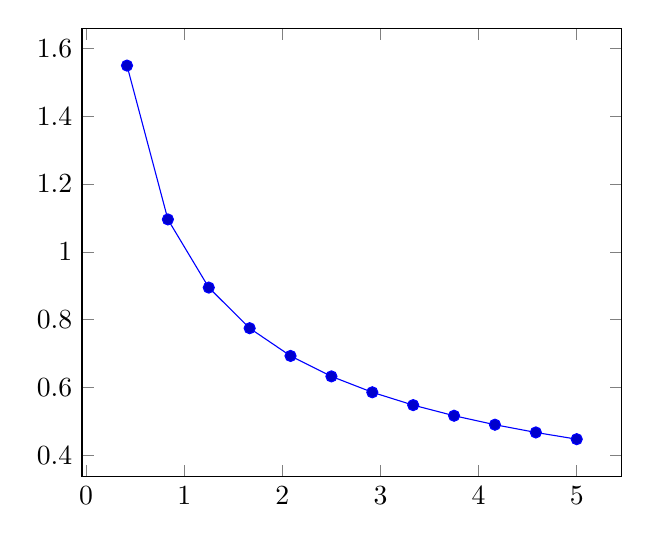
\begin{tikzpicture}
              \begin{axis}%[
                  %       xlabel=$x$,
                  %       ylabel={$y$}
                  %   ]
                  \addplot {1/sqrt(x)};
              \end{axis}
          \end{tikzpicture}
\end{itemize}

Ora ci chiediamo se il prodotto di due funzioni che appartengono a $L^1$ sta
ancora in $L^1$. Prendiamo dunque:

$$
    f(x) \cdot f(x) = \frac{1}{x}
$$

e verifichiamo se $\frac{1}{x} \in L^1(]0, 1])$:

\begin{equation}
    \begin{aligned}
        \int_{0}^{1} \frac{1}{x} \ dx & = \lim_{x \rightarrow 0^+} \int_{x}^{1} \frac{1}{t} \ dt = \lim_{x \rightarrow 0^+} [log |t|]_{0}^{1} = \\
                                      & = \lim_{x \rightarrow 0^+} [log 1 - log|x|] = +\infty.
    \end{aligned}
\end{equation}

Deduciamo quindi che non sempre il prodotto di due funzioni che stanno in $L^1$
appartiene a $L^1$.

\paragraph{Note:}
\begin{itemize}
    \item Ricordiamo che $log 1 = 0$
    \item Ricordiamo che $log |x|$ con $x$ che tende a $0^+$ (tende a 0 dalla
          destra) va a $-\infty$

          \begin{tikzpicture}
              \begin{axis}%[
                  %       xlabel=$x$, ylabel={$y$}
                  %   ]
                  \addplot {ln(x)};
              \end{axis}
          \end{tikzpicture}
    \item $\lim_{x \rightarrow 0^+} [log 1 - log|x|] = 0 - (-\infty) = +\infty$
\end{itemize}

Per far sì che il prodotto appartenga a $L^1$ dobbiamo introdurre il concetto di
\textit{\textbf{Prodotto di Convoluzione}}.

\section{Prodotto di Convoluzione}

La \textit{Convoluzione} è una tecnica che consente di regolarizzare le funzioni
e di approssimarle in $L^p$.
\begin{definition}
    Siano $f \in L^1(\mathbb{R})$ e $g \in L^p(\mathbb{R})$ con $1 \leq p \leq +\infty$.
    Allora possiamo definire il prodotto di convoluzione tra $f$ e $g$ come:

    $$
        \left( f \star g\right)(x) = \int_{\mathbb{R}} f(x - y) g(y) \ dy
    $$

    Risulta inoltre $f \star g \in L^p(\mathbb{R})$ e

    $$
        ||f \star g||_p \leq ||f||_1 \ ||g||_p.
    $$
\end{definition}

Diamo ora il seguente lemma riassuntivo che raccoglie tutte le principali
proprietà del prodotto di convoluzione.

\begin{lemma}
    Date $f, g, h \in L^1(\mathbb{R})$, risulta:

    \begin{enumerate}
        \item $f \star g = g \star f$ (proprietà commutativa);
        \item $f \star (g + h) = (f \star g) + (f \star h)$ (proprietà distributiva rispetto ala somma);
        \item $(f \star g) \star h = f \star (g \star h)$ (proprietà associativa);
        \item posto $\tau_a f(x) := f(x + a), \ x \in \mathbb{R}$ (operatore di traslazione,)
              risulta:
              $$
                  \tau_a (f \star g) = (\tau_a f) \star g
              $$
              (invarianza per traslazioni).
    \end{enumerate}
\end{lemma}

\section{Trasformata di Fourier}

In questa sezione daremo la definizione e richiameremo alcune importanti
proprietà che riguardano la trasformata di Fourier. La trasformata di Fourier
viene introdotta per poter dare una rappresentazione simile a quella fornita
dalle serie di Fourier per le funzioni non periodiche.

\begin{definition}
    % TODO: aggiungere ??
    %  f (una funzione che rappresenta un segnale) 
    Sia $f \in L^1(\mathbb{R})$. Allora la trasformata di Fourier di $f$ è
    definita come:

    $$
        \hat{f}(\lambda) := \int_{-\infty}^{+\infty} f(x) e^{-i\lambda x} \ dx, \ \lambda \in \mathbb{R}
    $$
\end{definition}

\paragraph{Note:}
\begin{itemize}
    \item Ricordiamo che $e^{-i\lambda x} = \cos(\lambda x) - i \sin(\lambda x)$
    \item Ricordiamo i numeri complessi definiti come:
          $$
              z = a + ib
          $$
          dove $a$ viene detta \textit{parte intera} e $b$ la \textit{parte immaginaria}.
    \item Il modulo di un numero complesso è definito come:
          $$
              |z| = \sqrt{a^2 + b^2}
          $$
          \begin{center}
              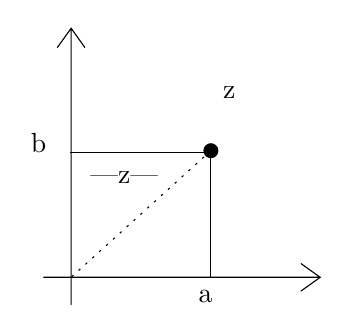
\begin{tikzpicture}[x=1.0pt,y=1.0pt,yscale=-1,xscale=1]
                  %uncomment if require: \path (0,300); %set diagram left start at 0, and has height of 300

                  %Straight Lines [id:da5730343469684522] 
                  \draw    (150.5,189.75) -- (150.5,234.75) ;
                  %Straight Lines [id:da70665287162995] 
                  \draw    (99.5,189.75) -- (150.5,189.75) ;
                  %Shape: Axis 2D [id:dp7340131235297938] 
                  \draw  (90,235) -- (190,235)(100,145) -- (100,245) (183,230) -- (190,235) -- (183,240) (95,152) -- (100,145) -- (105,152)  ;
                  %Shape: Circle [id:dp17035889321633024] 
                  \draw  [fill={rgb, 255:red, 0; green, 0; blue, 0 }  ,fill opacity=1 ] (148,189.25) .. controls (148,187.87) and (149.12,186.75) .. (150.5,186.75) .. controls (151.88,186.75) and (153,187.87) .. (153,189.25) .. controls (153,190.63) and (151.88,191.75) .. (150.5,191.75) .. controls (149.12,191.75) and (148,190.63) .. (148,189.25) -- cycle ;
                  %Straight Lines [id:da11421787184111976] 
                  \draw  [dash pattern={on 0.84pt off 2.51pt}]  (150.5,189.25) -- (100,235) ;

                  % Text Node
                  \draw (154,165) node [anchor=north west][inner sep=0.75pt]   [align=left] {z};
                  % Text Node
                  \draw (145,239) node [anchor=north west][inner sep=0.75pt]   [align=left] {a};
                  % Text Node
                  \draw (84.5,182) node [anchor=north west][inner sep=0.75pt]   [align=left] {b};
                  % Text Node
                  \draw (106,196) node [anchor=north west][inner sep=0.75pt]   [align=left] {|z|};


              \end{tikzpicture}
          \end{center}
    \item Quindi
          $$
              |e^{-i \lambda x}| = (\cos^2 (\lambda x) + \sin^2(\lambda x))^{\frac{1}{2}} = 1
          $$

\end{itemize}

Ci domandiamo il perchè sia così importante che $f \in L^1(\mathbb{R})$ (possibile domanda di esame).\\

\begin{center}
    Se $f \in L^1(\mathbb{R})$ allora $\hat{f} \in L^1(\mathbb{R})$.
\end{center}

\begin{proof}
    Poiché $f \in L^1(\mathbb{R})$, la funzione $\hat{f}(\lambda)$ risulterà sicuramente ben definita, infatti:

    \begin{equation}
        \begin{aligned}
            |\hat{f}(\lambda)| & = \left|\int_{\mathbb{R}} f(t) e^{-i \lambda t} \ dt \right| \leq \int_{\mathbb{R}} |f(t) e^{-i \lambda t}| \ dt =                  \\
                               & = \int_{\mathbb{R}} |f(t)| \cdot |e^{-i \lambda t}| \ dt = \int_{\mathbb{R}} |f(t)| \ dt < + \infty, \forall \lambda \in \mathbb{R}
        \end{aligned}
    \end{equation}

\end{proof}

%% TODO: la successiva parte che riguarda il grafico del segnale non l'ho capita.